%============================================================
% MTH 112Z Project - Supplement Angles
% Updated 202302
%============================================================

\section{Non-unit Circles} \label{supplement-nonunit-circles}
In this Section, we will learn some things.

\subsection*{Generalized Definitions of Trigonometric Functions}

        We can generalize the definitions of the trigonometric functions so that they are applicable to circles of any size.
      
        \begin{myDefinition} xml:id="definition-sincos">
        <statement>
          
            If the point $ P = \left(x,y \right)$ is specified by the angle $\theta$ on the circumference of a circle of radius $r$, then $ \cos (\theta ) = \frac{x}{r} $ and $ \sin (\theta ) = \frac{y}{r} $.
          
          \begin{center}
     \label{fig:nonunitcirclexy}
            \captionsetup{type=figure} \captionof{figure}{}
            <image width="50%">
              %<description>This is circle with radius r intersecting the terminal side of an angle labeled theta. The intersecting point is labeled P.</description>
              
                \begin{tikzpicture}
                  \begin{axis}[
                      width=8cm,
                      grid=none,
                      ticks=none,
                      trig format plots=rad,
                      axis equal,
                      xmin=-11,
                      xmax=11,
                      ymin=-11,
                      ymax=11,
                    ]
                    \addplot[angle, domain=0:pi/3, samples=50] ({1.5*cos(x)}, {1.5*sin(x)}) node[pos=0.5, above right, inner sep=1pt] {$\theta$};
                    \addplot[ray, -, black] coordinates {(0,0) (4,6.93)} node[pos=0.5, above left, inner sep=1pt] {$r$};
                    \addplot[soliddot] coordinates{(4,6.93)} node[above right] {$P=(x,y)$};
                    \addplot[domain=0:2*pi, samples=100] ({8*cos(x)},{8*sin(x)});
                  \end{axis}
                \end{tikzpicture}
              
            
          \end{center}
        </statement>
      \end{myDefinition}
      
        Notice that if we are on a unit circle, where $r=1$, then these definitions for $\cos(\theta)$ and $\sin(\theta)$ simplifly accordingly:
      
      
        <me>  \cos(\theta)=\frac{x}{r}=\frac{x}{1}=x  </me>
        <me>  \sin(\theta)=\frac{y}{r}=\frac{y}{1}=y  </me>
      

      
        We can use \ref{definition-sincos} to express the other four trigonometric functions in terms of $x$, $y$, and $r$.
      
      <sbsgroup>
        <sidebyside valign="top">
           
             \begin{align*}
                \tan(\theta) &= \frac{\sin(\theta)}{\cos(\theta)}  \\
                &= \frac{y/r}{x/r} \\
                &= \frac{y}{x} \\
             \end{align*}
           
           
             \begin{align*}
                \csc(\theta) &= \frac{1}{\sin(\theta)} \\
                &= \frac{1}{y/r} \\
                &= \frac{r}{y} \\
             \end{align*}
           
        </sidebyside>
        <sidebyside valign="top">
          
            \begin{align*}
               \sec(\theta) &= \frac{1}{\cos(\theta)} \\
               &= \frac{1}{x/r} \\
               &= \frac{r}{x} \\
            \end{align*}
          
          
            \begin{align*}
               \cot(\theta) &= \frac{1}{\tan(\theta)} \\
               &= \frac{1}{y/x} \\
               &= \frac{x}{y} \\
            \end{align*}
          
        </sidebyside>
      </sbsgroup>
      
        We summarize this in the following definition.
      
      \begin{myDefinition}  xml:id="definition-sixtrig">
        <statement>
          
            If the point $ P = \left(x,y \right)$ is specified by the angle $\theta$ on the circumference of a circle of radius $r$, then we can define the six trigonometric functions as follows.
          
          <sbsgroup>
            <sidebyside>
              
                <me> \cos (\theta ) = \frac{x}{r} </me>
              
              
                <me> \sin (\theta ) = \frac{y}{r} </me>
              
              
                <me> \tan (\theta ) = \frac{y}{x} </me>
              
            </sidebyside>
            <sidebyside>
              
                <me> \sec (\theta ) = \frac{r}{x} </me>
              
              
                <me> \csc (\theta ) = \frac{r}{y} </me>
              
              
                <me> \cot (\theta ) = \frac{x}{y} </me>
              
            </sidebyside>
          </sbsgroup>
          \begin{center}
     \label{fig:nonunitcirclexyallsix}
            \captionsetup{type=figure} \captionof{figure}{}
            <image width="50%">
              %<description> This is circle with radius r intersecting the terminal side of an angle in standard position labeled theta. The intersecting point is labeled P.</description>
              
                \begin{tikzpicture}
                  \begin{axis}[
                      width=8cm,
                      grid=none,
                      ticks=none,
                      trig format plots=rad,
                      axis equal,
                      xmin=-11,
                      xmax=11,
                      ymin=-11,
                      ymax=11,
                    ]
                    \addplot[angle, domain=0:pi/3, samples=50] ({1.5*cos(x)}, {1.5*sin(x)}) node[pos=0.5, above right, inner sep=1pt] {$\theta$};
                    \addplot[ray, -, black] coordinates {(0,0) (4,6.93)} node[pos=0.5, above left, inner sep=1pt] {$r$};
                    \addplot[soliddot] coordinates{(4,6.93)} node[above right] {$P=(x,y)$};
                    \addplot[domain=0:2*pi, samples=100] ({8*cos(x)},{8*sin(x)});
                  \end{axis}
                \end{tikzpicture}
              
            
          \end{center}
        </statement>
      \end{myDefinition}
      <example>
        <statement>
          
            Find the exact value of each of the six trigonometric functions of an angle $\theta$ if $(-1,2)$ is a point on its terminal side.
          
          \begin{center}
     \label{fig:nonunitcirclenegonetwo}
          \captionsetup{type=figure} \captionof{figure}{}
            <image width="50%">
              %<description>This is circle intersecting the terminal side of an angle labeled theta. The intersecting point has coordinates -1,2.</description>
              
                  \begin{tikzpicture}
                    \begin{axis}[
                        width=8cm,
                        grid=none,
                        ticks=none,
                        trig format plots=rad,
                        axis equal,
                        xmin=-4,
                        xmax=4,
                        ymin=-4,
                        ymax=4,
                      ]
                      \addplot[angle, domain=0:2.034, samples=50] ({0.5*cos(x)}, {0.5*sin(x)}) node[pos=0.5, above right, inner sep=1pt] {$\theta$};
                      \addplot[ray, -, black] coordinates {(0,0) (-1,2)} node[pos=0.5, below left, inner sep=1pt] {$r$};
                      \addplot[soliddot] coordinates{(-1,2)} node[above left] {$(-1,2)$};
                      \addplot[domain=0:2*pi, samples=100] ({2.236*cos(x)},{2.236*sin(x)});
                    \end{axis}
                  \end{tikzpicture}
                
              
            \end{center}
        </statement>
        <solution>
          
            We need the values of $x$, $y$, and $r$ to determine the exact value of each of the trigonemtric function. We are given $x$ and $y$, but will need to find the value of $r$.
          
          <sidebyside valign="middle" widths="78% 12%" margins="0% 5%">
            
              We can think of $r$ as the hypotenuse of a right triangle whose horiztonal leg has a length of $|-1|=1$ unit and vertical leg has a length of $2$ units. We can use the Pythagorean Theorem to solve for $r$:
                \begin{align*}
                   r^2 &= 1^2+2^2 \\
                   r^2 &= 5 \\
                   r &= \sqrt{5} \\
                \end{align*}
            
            
              
                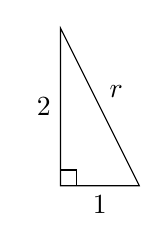
\begin{tikzpicture}
                  \draw (0,0) -- node[pos=0.5, below]{$1$} (-1,0) -- node[pos=0.5, left]{$2$} (-1,2) -- node[pos=0.5, above right]{$r$} cycle;
                  \draw (-0.8,0) |- (-1,0.2);
                \end{tikzpicture}
              
            
          </sidebyside>
          
            Now that we have values for $x$, $y$, and $r$, we can use \ref{definition-sixtrig} to state the exact values of each trigonometric function.
          
          <sbsgroup>
            <sidebyside valign="top">
              
                \begin{align*}
                   \cos(\theta) &= \frac{x}{r} \\
                   &= \frac{-1}{\sqrt{5}} \\
                   &= \frac{-1}{\sqrt{5}} \cdot \frac{\sqrt{5}}{\sqrt{5}} \\
                   &= -\frac{\sqrt{5}}{5} \\
                \end{align*}
              
              
                \begin{align*}
                   \sin(\theta) &= \frac{y}{r} \\
                   &= \frac{2}{\sqrt{5}} \\
                   &= \frac{2}{\sqrt{5}} \cdot \frac{\sqrt{5}}{\sqrt{5}} \\
                   &= \frac{2\sqrt{5}}{5} \\
                \end{align*}
              
            </sidebyside>
            <sidebyside valign="top">
              
                \begin{align*}
                   \tan(\theta) &= \frac{y}{x} \\
                   &= \frac{2}{-1} \\
                   &= -2 \\
                \end{align*}
              
              
                \begin{align*}
                   \sec(\theta) &= \frac{r}{x} \\
                   &= \frac{\sqrt{5}}{-1} \\
                   &= -\sqrt{5} \\
                \end{align*}
              
            </sidebyside>
            <sidebyside valign="top">
              
                \begin{align*}
                   \csc(\theta) &= \frac{r}{y} \\
                   &= \frac{\sqrt{5}}{2} \\
                \end{align*}
              
              
                \begin{align*}
                   \cot(\theta) &= \frac{x}{y} \\
                   &= \frac{-1}{2} \\
                   &= -\frac{1}{2} \\
                \end{align*}
              
            </sidebyside>
          </sbsgroup>
        </solution>
      </example>

      
        We can use \ref{definition-sincos} to express the coordinates of point $P$ inFigure \ref{fig:nonunitcirclexy}. We do this by solving the equations $ \cos (\theta ) = \frac{x}{r} $ and $ \sin (\theta ) = \frac{y}{r} $ for $x$ and $y$, respectively:
      
      
          <me> \cos(\theta)=\frac{x}{r} \implies x=r\cos(\theta) </me>
          <me> \sin(\theta)=\frac{y}{r} \implies y=r\sin(\theta) </me>

      
      
        We summarize this below.
      
      \begin{myDefinition}  xml:id="definition-coordinates">
        <statement>
          
            If the point $ P = \left(x,y \right)$ is specified by the angle $\theta$ on the circumeference of a circle of radius $r$, then
            $x=r \cos (\theta )$ and $y=r \sin (\theta )$.
          
          \begin{center}
     \label{fig:nonunitcircletrig}
            \captionsetup{type=figure} \captionof{figure}{}
            <image width="50%">
              %<description>This is circle with radius r intersecting the terminal side of an angle theta. The intersecting point labeled P.</description>
              
                \begin{tikzpicture}
                  \begin{axis}[
                      width=8cm,
                      grid=none,
                      ticks=none,
                      trig format plots=rad,
                      axis equal,
                      xmin=-11,
                      xmax=11,
                      ymin=-11,
                      ymax=11,
                      clip=false,
                    ]
                    \addplot[angle, domain=0:pi/3, samples=50] ({1.5*cos(x)}, {1.5*sin(x)}) node[pos=0.5, above right, inner sep=1pt] {$\theta$};
                    \addplot[ray, -, black] coordinates {(0,0) (4,6.93)} node[pos=0.5, above left, inner sep=1pt] {$r$};
                    \addplot[soliddot] coordinates{(4,6.93)} node[above right] {$P=(r\cos(\theta),r \sin (\theta ))$};
                    \addplot[domain=0:2*pi, samples=100] ({8*cos(x)},{8*sin(x)});
                  \end{axis}
                \end{tikzpicture}
              
            
          \end{center}
        </statement>
      \end{myDefinition}

      <example>
        <statement>
          
            Find the coordinates of the point on a circle with a radius of $8$ units corresponding to an angle of $\frac{7\pi}{4}$.
          
          \begin{center}
     \label{fig:nonunitcirclegivenangleandrad}
          \captionsetup{type=figure} \captionof{figure}{}
            <image width="50%">
              %<description>This is circle a circle of radius 8 intersecting the terminal side of the angle 7 time pi over 4 in standard position.</description>
              
                  \begin{tikzpicture}
                    \begin{axis}[
                        width=8cm,
                        grid=none,
                        ticks=none,
                        trig format plots=rad,
                        axis equal,
                        xmin=-11,
                        xmax=11,
                        ymin=-11,
                        ymax=11,
                      ]
                      \addplot[angle, domain=0:7*pi/4, samples=50] ({1.5*cos(x)}, {1.5*sin(x)}) node[pos=0.5, above left, inner sep=0pt] {$\frac{7\pi}{4}$};
                      \addplot[ray, -, black] coordinates {(0,0) (5.657,-5.657)} node[pos=0.5, below left, inner sep=1pt] {$8$};
                      \addplot[soliddot] coordinates{(5.657,-5.657)};
                      \addplot[domain=0:2*pi, samples=100] ({8*cos(x)},{8*sin(x)});
                    \end{axis}
                  \end{tikzpicture}
                
              
            \end{center}
        </statement>
        <solution>
          
            We are given the values of $r$ and $\theta$, so we can use \ref{definition-coordinates} to determine the coordinate values.
          
          
            Find $x$:
              \begin{align*}
                 x &= r\cos\left( \theta \right)\\
                 &= 8\cos\left( \frac{7\pi}{4}\right)\\
                 &= 8 \cdot \frac{\sqrt{2}}{2} \\
                 &= 4\sqrt{2} \\
              \end{align*}
          
          
            Find $y$:
            \begin{align*}
               y &= r\sin\left( \theta \right)\\
               &= 8\sin\left( \frac{7\pi}{4}\right)\\
               &= 8 \left( -\frac{\sqrt{2}}{2} \right)\\
               &= -4\sqrt{2} \\
            \end{align*}
          
          
            So the coordinates of the point on a circle with a radius of $8$ units corresponding to an angle of $\frac{7\pi}{4}$ are $\left( 4\sqrt{2}, -4\sqrt{2} \right)$.
          
        </solution>
      </example>
      <exercises xml:id="exercises-nonunit-circles">
      <!-- #1 from Word Version - Part 3 -->
          <exercisegroup  cols="2"  xml:id="exercisegroup-six-trig-values">
            \subsection*{Six Trigonemtric Function Values}
              
                  In <xref ref="exercisegroup-six-trig-values" text="local">Exercises</xref>, find the exact value of each of the six trigonometric functions of an angle $\theta$ if the given point is on its terminal side.
                  
              
              <exercise>
                  <statement>
                      
                        $(3,4)$
                      
                  </statement>
                  <answer>
                    
                      \begin{align*}
                         \cos(\theta) &= \frac{3}{5} \\
                         \sin(\theta) &= \frac{4}{5} \\
                         \tan(\theta) &= \frac{4}{3} \\
                         \sec(\theta) &= \frac{5}{3} \\
                         \csc(\theta) &= \frac{5}{4} \\
                         \cot(\theta) &= \frac{3}{4} \\
                      \end{align*}
                    
                  </answer>
              </exercise>
              <exercise>
                  <statement>
                      
                        $(-2,-6)$
                      
                  </statement>
                  <answer>
                    
                      \begin{align*}
                         \sin(\theta) &= -\frac{\sqrt{10}}{10} \\
                         \cos(\theta) &= -\frac{3\sqrt{10}}{10} \\
                         \tan(\theta) &= 3 \\
                         \sec(\theta) &= -\sqrt{10} \\
                         \csc(\theta) &= -\frac{\sqrt{10}}{3} \\
                         \cot(\theta) &= \frac{1}{3} \\
                      \end{align*}
                    
                  </answer>
              </exercise>
          </exercisegroup>
          <exercisegroup  cols="2"  xml:id="exercisegroup-coordinates">
            \subsection*{Find the coordinates}
              
                  In <xref ref="exercisegroup-coordinates" text="local">Exercises</xref>, find the coordinates of the point on a circle with the given radius corresponding to the given angle.
                  
              
              <exercise>
                  <statement>
                      
                        $r=3, \theta=\frac{7\pi}{6}$
                      
                  </statement>
                  <answer>
                    
                      $\left( -\frac{3\sqrt{3}}{2}, -\frac{3}{2} \right)$
                    
                  </answer>
              </exercise>
              <exercise>
                  <statement>
                      
                        $r=10, \theta=\frac{\pi}{3}$
                      
                  </statement>
                  <answer>
                    
                      $\left( 5, 5\sqrt{3} \right)$
                    
                  </answer>
              </exercise>
          </exercisegroup>
      </exercises>
</section>